\documentclass[ngerman]{gdb-aufgabenblatt}

\usepackage{enumitem}
\usepackage{dingbat}
\renewcommand{\Aufgabenblatt}{1}
\renewcommand{\Ausgabedatum}{Mi. 18.10.2017}
\renewcommand{\Abgabedatum}{Fr. 03.11.2017}
\renewcommand{\Gruppe}{Meimerstorf,Jochens,T�ter}
\renewcommand{\STiNEGruppe}{19}
\usepackage{tabularx}


\begin{document}

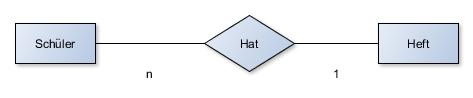
\includegraphics[scale=1]{RelationShipBeispiel.jpg} \ \\

Am Anfang kurz definiert wie die Relationen zu lesen sind. So wie es in der Vorlesung vorgestellt wurde. \\
1 Kind kann n Hefte haben. \\
Ein Heft kann nur von einem Kind bessen werden \\
\section{Informationsmodellierung mit dem Entity-Relationship Modell}
\subsection{}
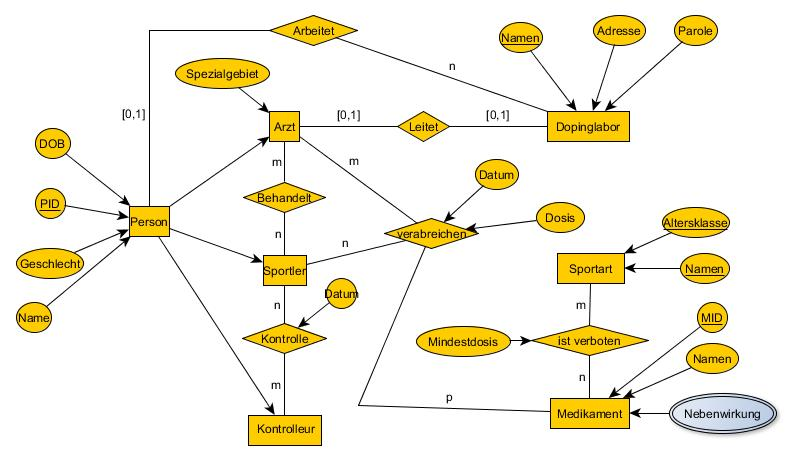
\includegraphics[scale=0.7]{GraphAufgabe2.jpg}
\subsection{}
Ein Medikament darf einem Sportler nicht verabreicht werden, wenn es in der Sportart verboten ist. \\
Ein Kontrolleur darf einen Sportler nicht am selben Tag kontrollieren wie ihm ein Medikament vera	breicht wird. \\
\section{Informationsmodellierung: Beschreibung mit ER-Modellen}
\subsection{}
Ein Fahrzeug hat eine eindeutige KFZ-Nr. sowie ein nicht eindeutigen Fahrzeugtyp. \\
Eine Person hat eine eindeutige SVNr. sowie einen nicht eindeutigen Namen. \\
Ein Fahrzeug ist auf eine Person gemeldet \\
Und Jede Person hat n Fahrzeuge gemeldet \\
\subsection{}
Ein Fahrzeug hat eine eindeutige KFZ-Nr. sowie ein nicht eindeutigen Fahrzeugtyp und kann genau einmal gekauft werden. \\
Ein Verk�ufe hat eine eindeutige VNr. sowie einen nicht eindeutigen Namen und kann m Verk�ufe t�tigen. \\
Ein Kunde hat eine eindeutige K-Nr. und kann n K�ufe t�tigen. \\
Ein Kauf hat ein Datum und einen Preis. \\
\subsection{}
Ein Superheld hat eine eindeutige HNr. sowieso einen Namen und ein Einsatzgebiet. Jeder Superheld besitzt n Superkr�fte \\
Eine Superkraft hat eine eindeutige Bezeichnung, sowie eine Beschreibung. Jede Superkraft wird von m Superhelden verwendet. \\
Jede Beziehung zwischen Superheld und Superkraft wird von einer Menge von  Bedingungen begleitet. \\
\subsection{}   
Eine Person hat eindeutige Kombination aus Vor und Nachnamen.\\
Ein Erz�hler ist eine Person \\
Ein Zuh�rer ist eine Person \\
Ein Erz�hler hat mind. eine Person dem er einen Witz erz�hlt\\
Ein Zuh�rer hat mind. 0 Erz�hler  \\
Einen Witz erz�hlen hat eine Menge von Pointen\\
\subsection{}
Ein Erz�hler kann max. einen Witz erz�hlen. und mindestens 0 \\
\section{}
\subsection{}
Minimal bedeutet, dass ein Schl�ssel nicht aus mehreren Attributen bestehen darf, wenn bereits eins dieser Attribute eindeutig ist. \\
Eindeutig bedeutet, dass das Attribut bzw. die Kombination aus mehreren Attributen nur maximal ein Mal	 in allen Entit�ten vorkommt. \\
Einige Attribute die man verwenden k�nnte, w�re das Geburtsdatum, dieses ist f�r unsere 6 Personen eindeutig und minimal. Weiterhin k�nnte man die Telefon Nr. verwenden. \\
Das Schl�sselpaar(Vorname,Nachname) ist nicht Minimal, da schon nur das Attribut Vorname eindeutig ist. \\
\subsection{} 
Im Allgemeinen ist das ganze Problem ein wenig schwerer, da auch unsere beiden M�glichen Schl�ssel in diesem Fall relativ wahrscheinlich nicht eindeutig sind. Bei den Geburtstagen siehe https://de.wikipedia.org/wiki/Geburtstagsparadoxon . Und auch bei den Telefonnummern, k�nnte es durchaus sein, dass zwei Studenten in derselben Wohnung leben(WG) oder Geschwister sind die noch Zuhause wohnen.\\
Dies l�sst sich, wenn wir keinerlei neue ID hinzuf�gen sollen am leichtesten mit einem Schl�sselpaar l�sen. In diesem Fall w�rden sich vermutlich (Telefon-Nr.,Geb-Datum,Vorname) anbieten, da bei nur Telefon-Nr. und Geb-Datum h�tten wir immernoch Zwillinge die noch Zuhause wohnen mit drin. Allerdings wenn wir noch den Vornamen dazunehmen, d�rfte die Wahrscheinlichkeit gegen 0 laufen. \\
\textbf{Allerdings} w�rde man das in der Praxis nat�rlich nicht verwenden, weil selbst eine kleine Wahrscheinlichkeit das ganze zusammenbrechen lassen k�nnte. Wir w�rden empfehlen hier die Einf�hrung einer Matrikelnummer zu veranlassen die eindeutig f�r jeden Studenten vergeben wird. \\
\end{document}